\documentclass{beamer}

% Prepare for svenska tecken
\usepackage[T1]{fontenc}
\usepackage[utf8]{inputenc}
\usepackage[swedish]{babel}
%\usepackage[]{geometry}
\addto\captionsswedish{\renewcommand{\figurename}{Bild}}
\usepackage{amsmath}
\usepackage{fancyhdr}
\usepackage{wrapfig}
\usepackage{caption}
\usepackage{framed}
\usepackage[fulladjust]{marginnote}
\usepackage{color}
\newcommand{\hilight}[1]{\colorbox{yellow}{#1}}
\usepackage{hyperref}
\hypersetup{
    colorlinks,
    citecolor=black,
    filecolor=black,
    linkcolor=black,
    urlcolor=black
}
\usepackage{stmaryrd} % För symbolen \boxbox, kräver paketet texlive-math-extra

% % % % % % % % % % % 
% Detta är nya environments för review. De bör vara relativt självförklarande hur de används.
% I princip sätter man bara den del av texten som har en viss status mellan\begin{rev-granskat} och \end{rev-granskat} tex.
% Undvik att nästla dem för det är ingen idé det fungerar inte.
% De är testade med ett antal andra environemnt som tabular mm men kolla att det fungerar med de environments du använder.
% % % % % % % % % % % % % % % % % % % % % % % % % % % % % % % % % % % % % % % % % % % % % % % % % % % % % % % % % % % % % % % 
%\usepackage[svgnames,rgb]{xcolor}
%\usepackage{pdfcomment}
%\newenvironment{rev-ogranskat}{\begin{pdfsidelinecomment}[color=black,linewidth=3px,caption=inline]{Ogranskat}}{\end{pdfsidelinecomment}}
%\newenvironment{rev-omarbetas}{\begin{pdfsidelinecomment}[color=red,linewidth=3px,caption=inline]{Omarbetas}}{\end{pdfsidelinecomment}}
%\newenvironment{rev-raderas}{\begin{pdfsidelinecomment}[color=red,linewidth=3px,caption=inline]{Raderas}}{\end{pdfsidelinecomment}}
%\newenvironment{rev-redo}{\begin{pdfsidelinecomment}[color=yellow,linewidth=3px,caption=inline]{Redo att granska}}{\end{pdfsidelinecomment}}
%\newenvironment{rev-granskat}[1][]%
%{\begin{pdfsidelinecomment}[color=green,linewidth=3px,caption=inline]%
%{Granskat #1}}%
%{\end{pdfsidelinecomment}}
%\newenvironment{rev-nytt}[1][]%
%{\begin{pdfsidelinecomment}[color=brown,linewidth=3px,caption=inline]%
%{Nytt #1}}%
%{\end{pdfsidelinecomment}}
%\newenvironment{rev-releasat}{\begin{pdfsidelinecomment}[color=blue,linewidth=3px,caption=inline]{Klart}}{\end{pdfsidelinecomment}}

%\clubpenalty=9990
%\widowpenalty=9999
%\brokenpenalty=4999

\usepackage[europeanvoltages,europeancurrents,europeanresistors,cuteinductors,smartlabels]{circuitikz}
\usepackage[framemethod=TikZ]{mdframed}

\mdfdefinestyle{FactBox}{%
    linecolor=blue,
    outerlinewidth=2pt,
    roundcorner=20pt,
    innertopmargin=\baselineskip,
    innerbottommargin=\baselineskip,
    innerrightmargin=20pt,
    innerleftmargin=20pt,
    backgroundcolor=gray!50!white}
\newcommand{\infobox}[1]{
\begin{wrapfigure}{r}{0.5\textwidth}
  \begin{mdframed}[style=FactBox]
#1
  \end{mdframed}
\end{wrapfigure}
}

% Make some unicode characters usable
\DeclareUnicodeCharacter{00B0}{\ensuremath{^\circ}} % unicode 00B0 ° degree sign
\DeclareUnicodeCharacter{00B5}{\ensuremath{\mu}} % unicode 00B5 µ micro sign
\DeclareUnicodeCharacter{03C0}{\ensuremath{\pi}} % unicode 3C0 π greek small letter pi
\DeclareUnicodeCharacter{03A9}{\ensuremath{\Omega}} % unicode 3A9 Ω greek capital letter omega
\DeclareUnicodeCharacter{2206}{\ensuremath{\Delta}} % unicode 2206 ∆ increment


% Prepare for tables
\usepackage{multirow}
\usepackage{longtable}

% Prepare for lists
%\usepackage{enumitem}

% Prepare for graphics
\usepackage{xspace,graphicx}

\raggedbottom


%% Frontpage bacground
\usepackage{eso-pic}
\newcommand\BackgroundPic{%
\put(0,0){%
\parbox[b][\paperheight]{\paperwidth}{%
\vfill
\centering
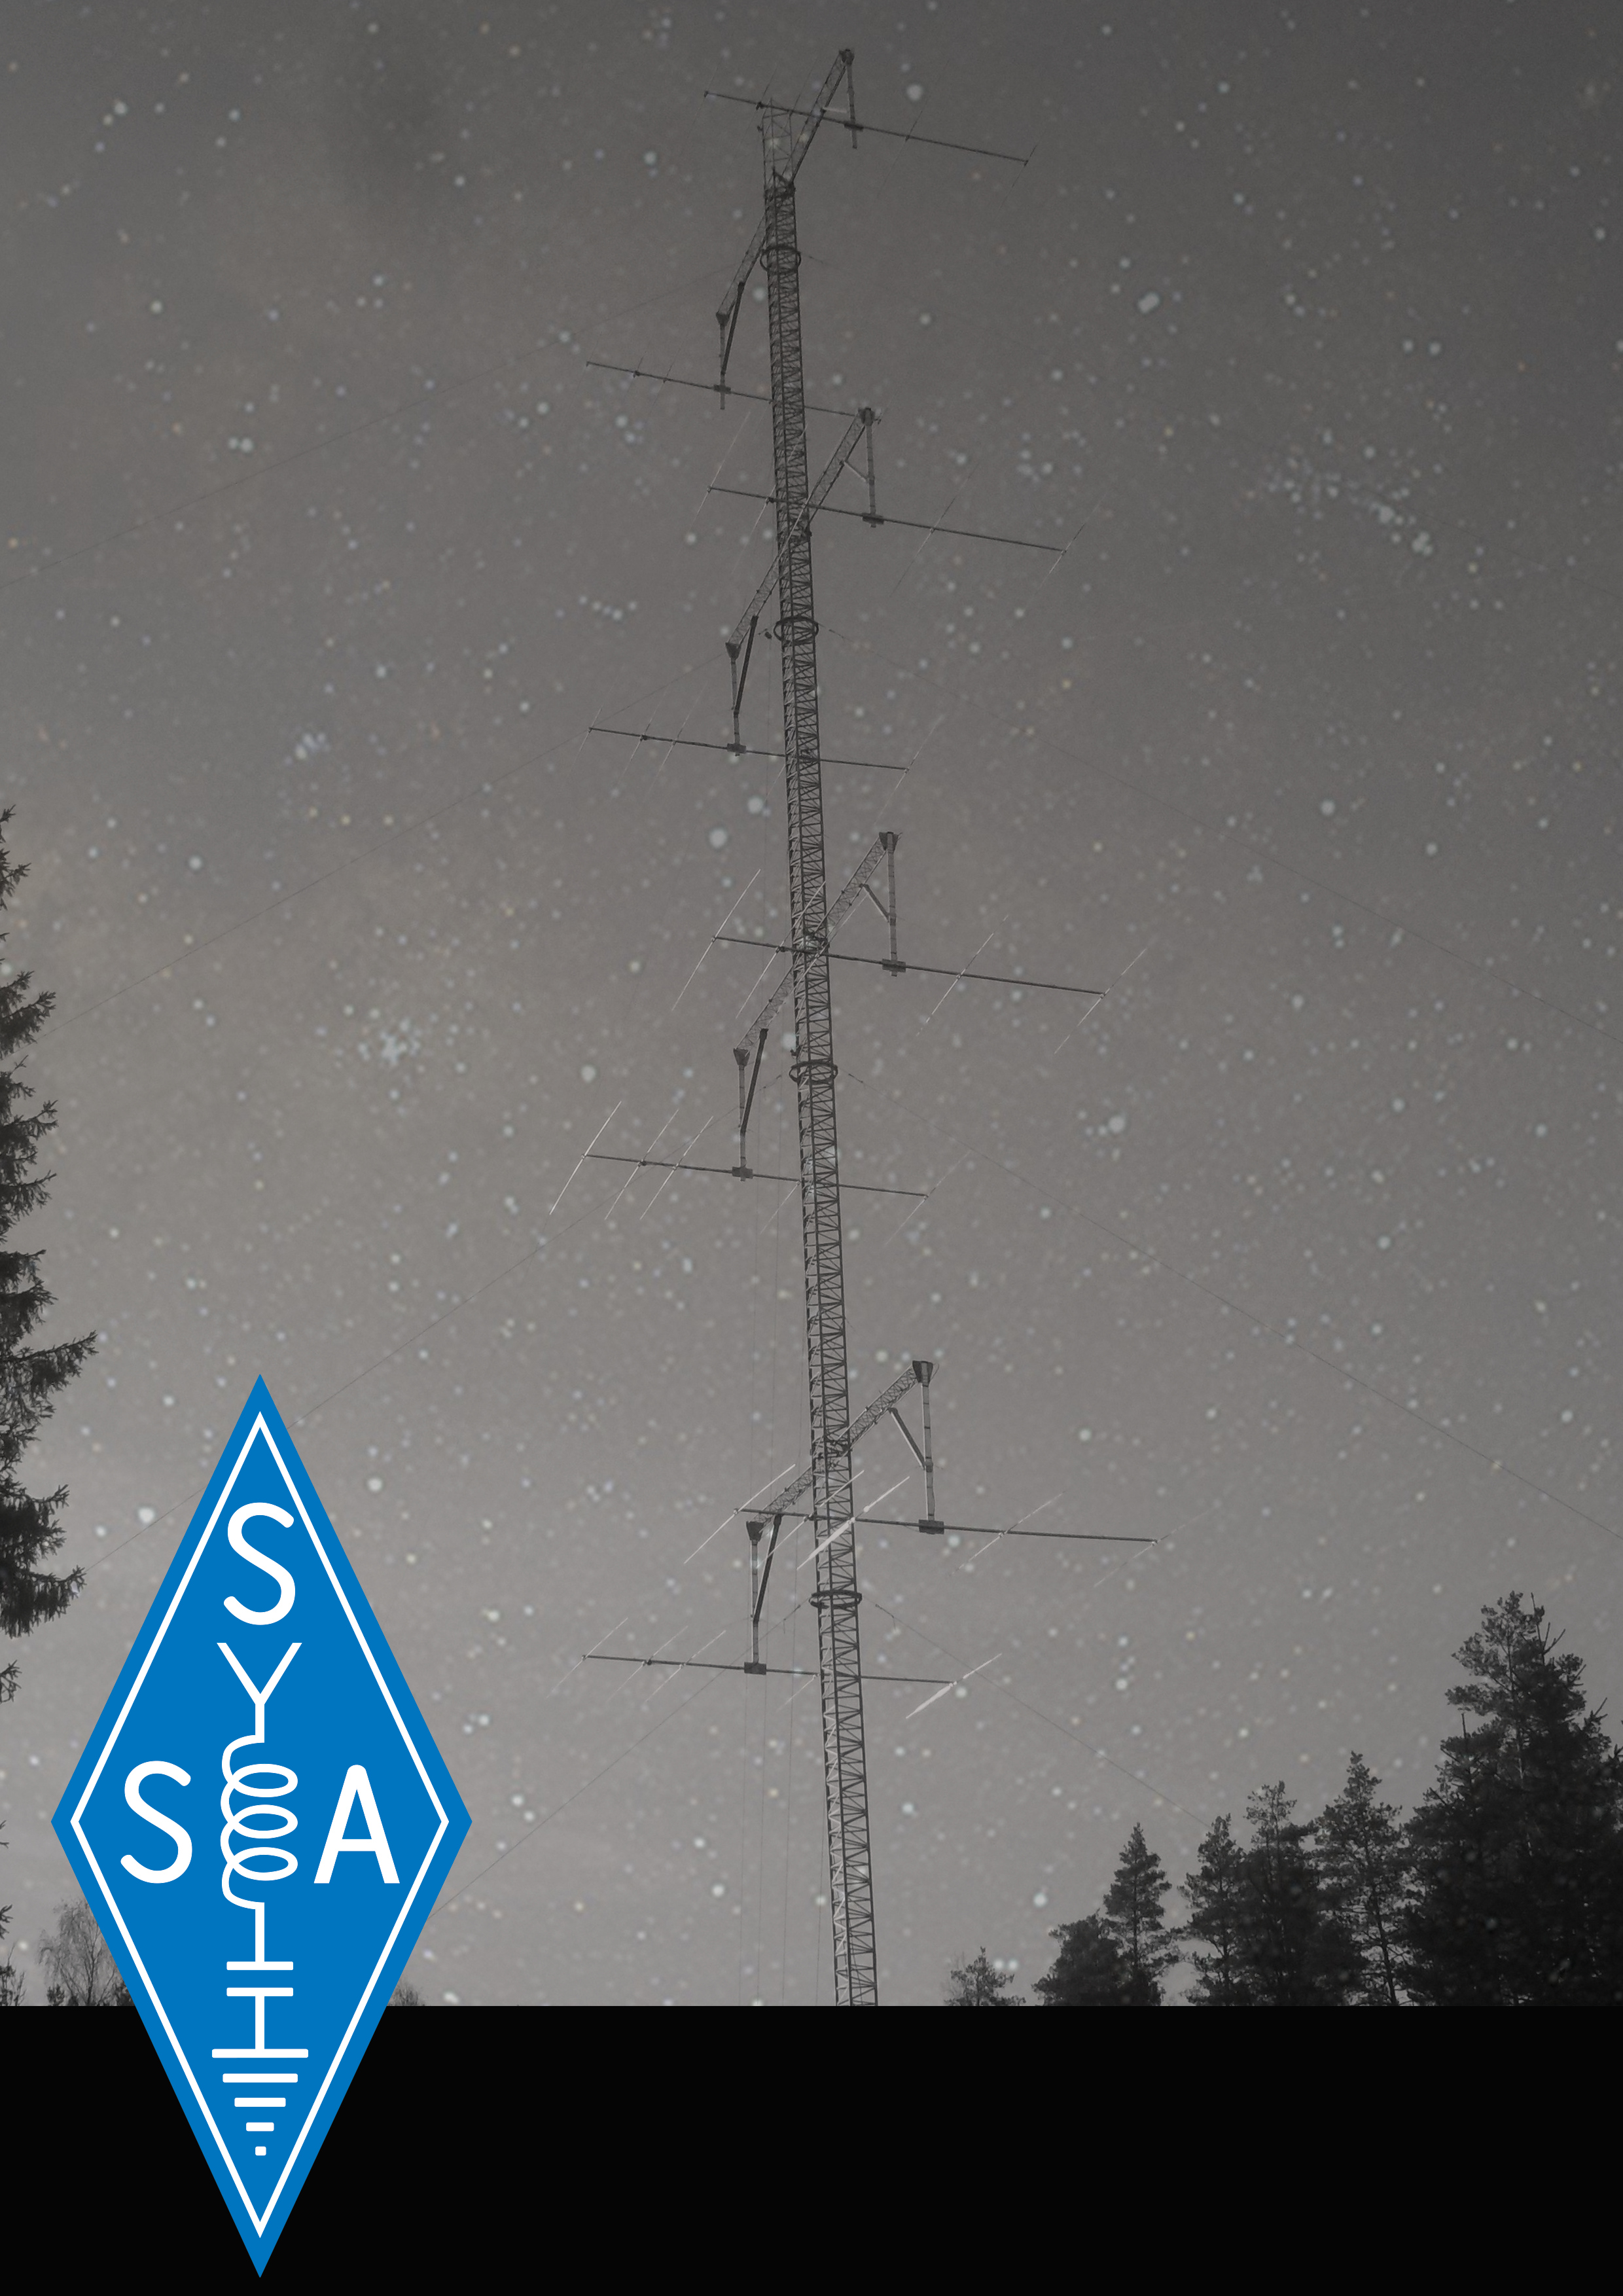
\includegraphics[width=\paperwidth,height=\paperheight,%
keepaspectratio]{images/koncept-front.jpg}%
\vfill
}}}


\newcommand\BackgroundPicLast{%
\put(0,0){%
\parbox[b][\paperheight]{\paperwidth}{%
\vfill
\centering

\includegraphics[width=\paperwidth,height=\paperheight,%
keepaspectratio]{images/koncept-back.pdf}%
\vfill
}}}

\usepackage[swedish]{babel}

\mode<presentation>
{
\usetheme{Madrid}
\usecolortheme{default}
\usefonttheme{serif}
\setbeamertemplate{navigation symbols}{}
\setbeamertemplate{caption}[numbered]
}
\usepackage{tikz}
\usepackage{amsmath,amsfonts,amssymb,bm,mathrsfs}
\usetikzlibrary{shapes,arrows}

\title{Växelström och reaktans}
\author{Magnus Danielson SA0MAD}

\begin{document}

\begin{frame}
\titlepage

\includegraphics[height=0.3\textheight]{images/ssalogo}
\end{frame}

\begin{frame}{Outline}
\tableofcontents
\end{frame}

\section{Växelström}

\begin{frame}{Sinuskurvan}

\begin{figure}[h]
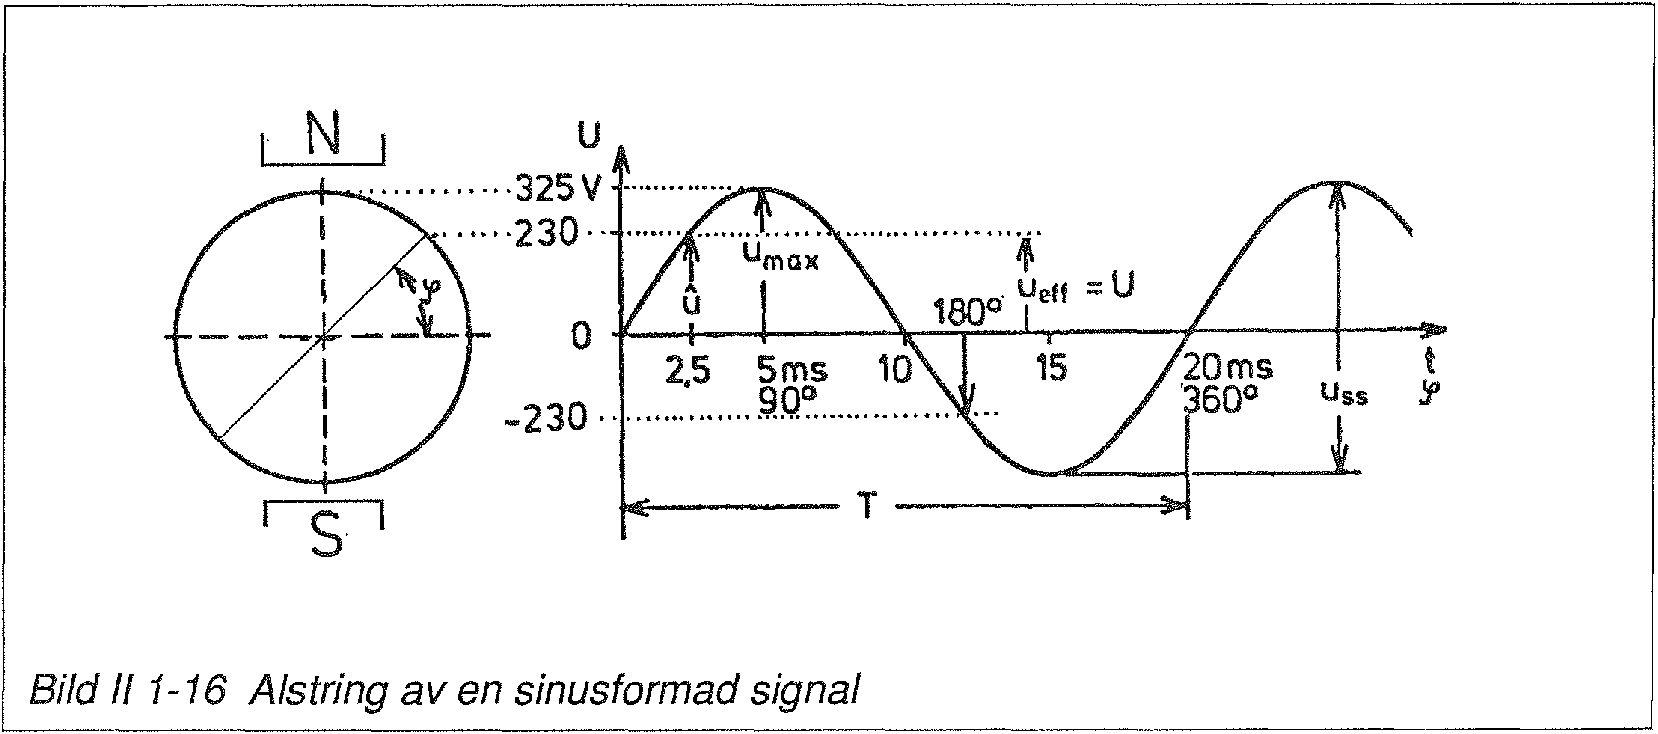
\includegraphics[width=0.8\textwidth]{images/bild_2_1-16}
%\caption{Alstring av en sinusformad signal}
\label{fig:BildII1-16}
\end{figure}

\begin{itemize}
\item Den grundläggande vågformen är sinus
\item Periodtiden $T$ är den tid det tar för en cykel.
\item Frekvensen $f$ är antalet cykler per sekund $f=\frac{1}{T}$
\item Toppvärdet $\hat{u}=u_{max}$ är amplituden av signalen
  \item Effektivvärdet (RMS) $U = $ är medeleffekten (som värmer ett motstånd lika mycket)
\end{itemize}
\end{frame}

\begin{frame}{Sinuskurvan - räkna tid}
  \begin{itemize}
  \item Periodtid anges i enheten sekund [s], dvs. antalet sekund för en period
  \item Frekvens anges i enheten Hertz [1/s], dvs. antalet perioder för en sekund
  \item Frekvensen $f$ ges av periodtiden $f = \frac{1}{T}$
  \item Periodtiden $T$ ges av frekvensen $T = \frac{1}{f}$
  \item Exempel: Elnätet har den nominella frekvensen $f=50\,Hz$ och periodtiden $T=\frac{1}{f}=\frac{1}{50}=20\,ms$
  \item Exempel: En frekvensreferens ger nominellt en periodtid på $T=100\,ns$ och därmed frekvensen $f=\frac{1}{T}=\frac{1}{100\cdot10^{-9}}=\frac{1}{10^{-7}}=10^7=10\,MHz$
  \end{itemize}
\end{frame}

\begin{frame}{Sinuskurvan - räkna amplitud}
  \begin{itemize}
  \item Momentanvärdet $u$ anger spänningen vid en vis tidpunkt
  \item Toppvärdet $\hat{u}$ anger den högsta spänningen som momentanvärdet får
  \item Effektivvärdet $U$ anger den spänning som motsvara samma effekt som sinusen motsvarar
  \item Toppvärdet $\hat{u}$ ges av effektivvärdet $\hat{u} = U\sqrt{2} \approx 1.414 U$
  \item Effektivvärdet (RMS) $U$ ges av toppvärdet $U = \frac{\hat{u}}{\sqrt{2}} \approx 0.707 \hat{u}$
  \item Topp-Toppvärdet $U_{PP}$ är det dubbla topp-värdet
  \item Exempel: Elnätet har nominellt effektivvärdet $U=230\,V$ och toppspänningen blir $\hat{u} = 1.414U = 1.414\cdot230 = 325.22\,V$
  \end{itemize}
\end{frame}

\section{Kondensator}

\begin{frame}{Kondensator}

\begin{figure}[h]
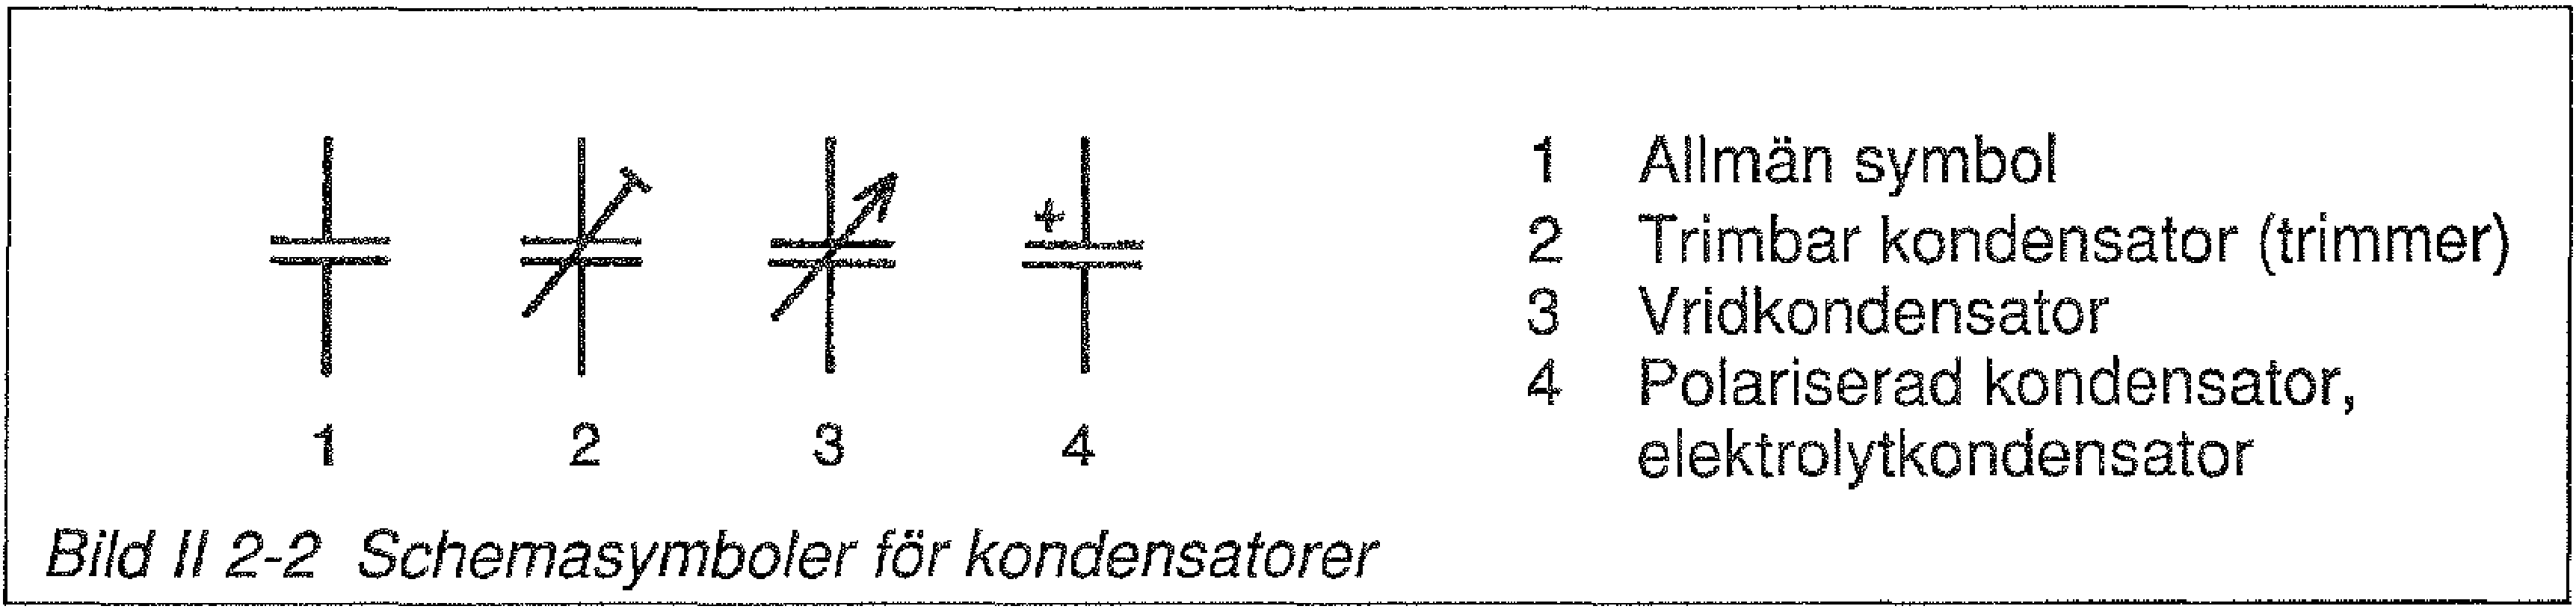
\includegraphics[width=\textwidth]{images/bild_2_2-02}
\end{figure}

\begin{itemize}
  \item Mellan två ledare med en laddning skapas ett elektriskt fält
  \item Förmågan att hålla en elektrisk laddning kallas för kapacitans $C$ och mäts i Farad [F]
  \item Den elektriska laddningen $Q$ mäts i Coulomb [1 C = 1 As], dvs. $Q=It$
  \item Spänningen $U$ beror på laddningen $Q$ och kapacitansen $C$ som $Q=CV$
\end{itemize}
\end{frame}

\begin{frame}{Kondensator värden}
  \begin{itemize}
    \item Kondensatorns värden är i allmänhet i $mF$, $\mu F$, $nF$ och $pF$
    \item Seriekoppling $\frac{1}{C_{tot}} = \frac{1}{C_1} + \frac{1}{C_2} + \ldots + \frac{1}{C_N}$
    \item Parallellkoppling $C_{tot} = C_1 + C_2 + \ldots + C_N$
    \item Minnesregel: samma formler som för motstånd - men tvärt om
  \end{itemize}
\end{frame}

\begin{frame}{Kondensator och växelström}
  \begin{itemize}
  \item Impedans $Z$ är förhållandet mellan ström och spänning $U=ZI$
  \item Reaktans $X$ är förhållandet mellan ström och spänning för en reaktans
  \item Reaktans från latinets re (åter) agere (verkan)
  \item Kondensatorns reaktans motverkar att spänningen ändras, då dess laddning har motsvarande Elektromotorisk Kraft (EMK)
  \item Reaktansen för en kondensator beror på kapacitansen $C$ och frekvensen $f$ enligt $X_C = \frac{1}{2\pi f C}$
  \item Fasförskjutning mellan ström och spänning är 90 grader före spänningen
  \item Överkurs-bonus: $Z = \frac{1}{sC} = \frac{1}{j\omega C} = \frac{-j}{2\pi f C} = -jX_C$
  \end{itemize}
\end{frame}

\begin{frame}{Kondensator}

\begin{figure}[h]
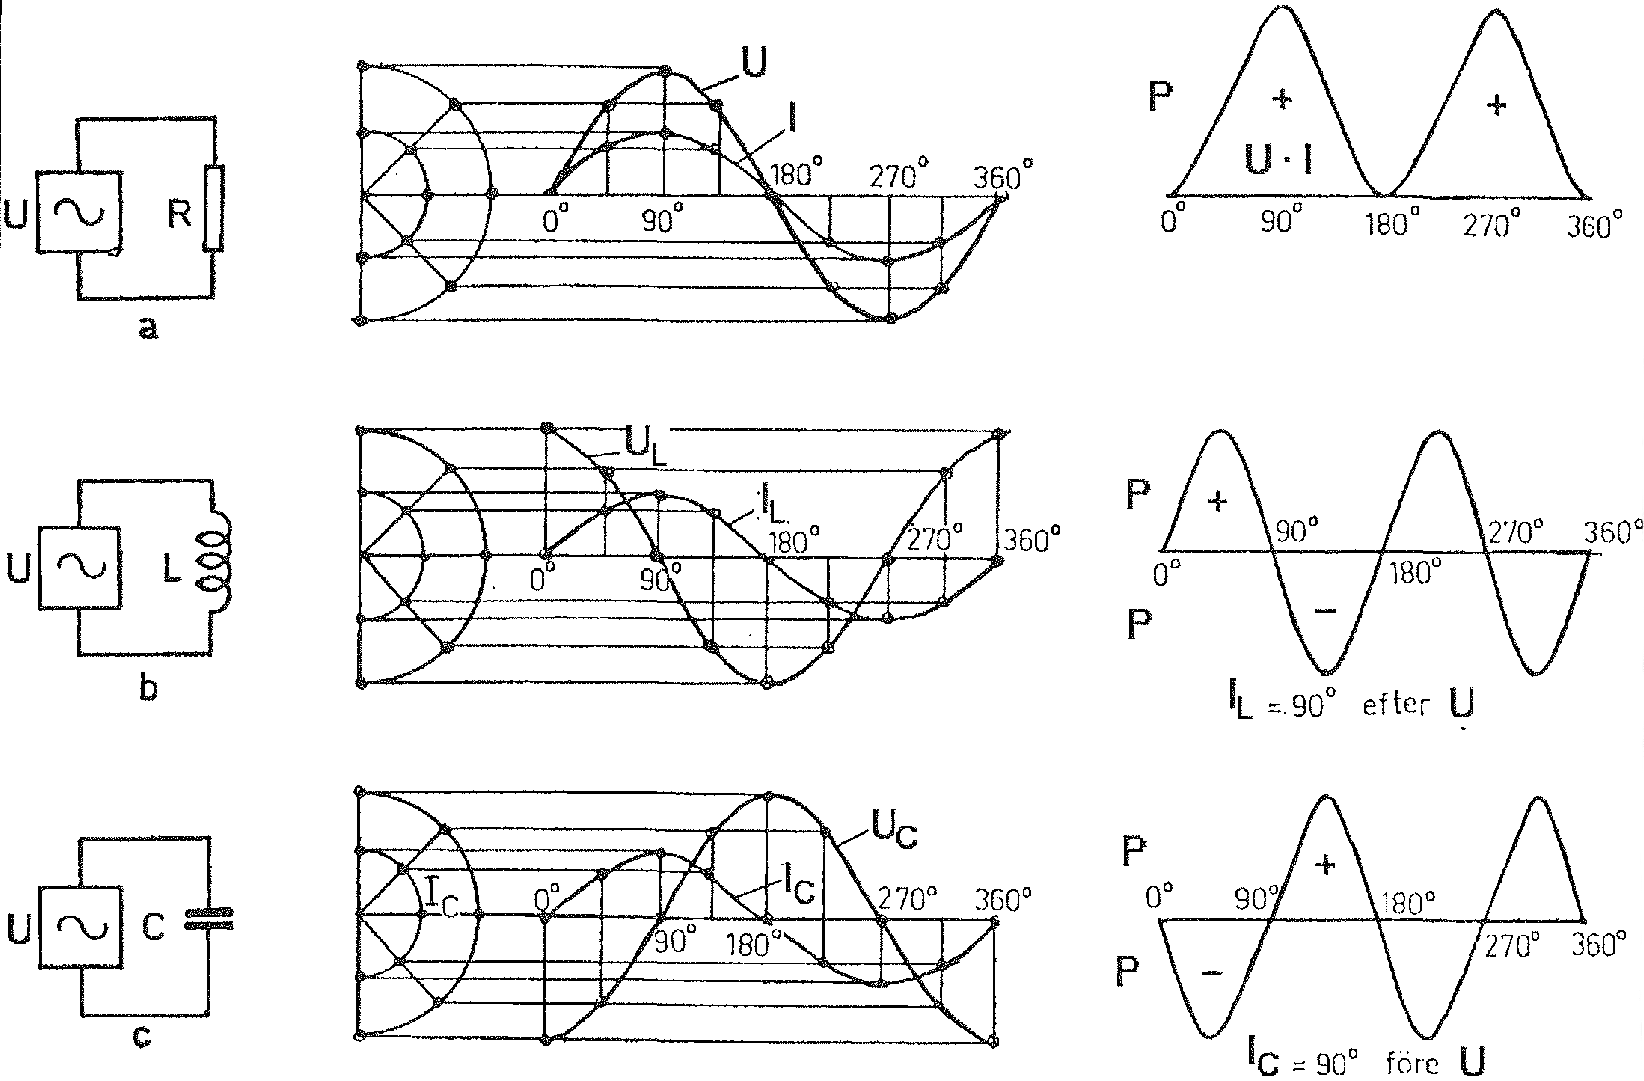
\includegraphics[width=0.8\textwidth]{images/bild_2_3-11}
\end{figure}

\end{frame}

\section{Spolar och induktans}

\begin{frame}{Induktans}

\begin{figure}[h]
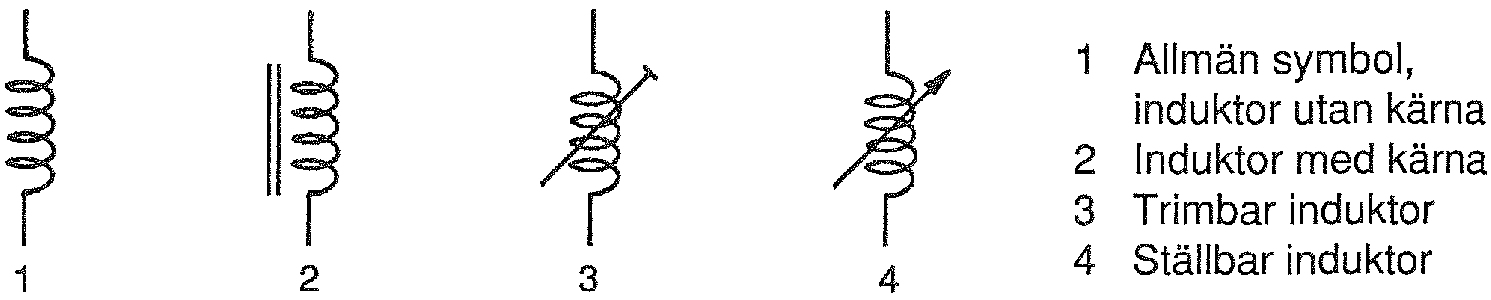
\includegraphics[width=\textwidth]{images/bild_2_2-04}
\end{figure}

\begin{itemize}
  \item En ström genom en ledare skapar ett magnetiskt fält
  \item Förmågan att hålla en magnetiskt fält kallas för induktans $L$ och mäts i Henry [H]
  \item Magnetisk fältstyrka $H$ i Ampere per meter [A/m] $H=\frac{\Theta}{l} = \frac{I \cdot N}{l}$
  \item Magnetisk flödestäthet $B$ i Tesla [T] (tidigare Gauss) $B = \mu \cdot H$
  \item Magnetisk flöde $\Phi$ i Weber eller Volt sekund [Vs] $\Phi = B \cdot A$
  \item Induktans $L$ gives ur $L=\frac{N\Phi}{I}$
\end{itemize}
\end{frame}

\begin{frame}{Induktorns värden}
  \begin{itemize}
    \item Induktorns värden är i allmänhet i $mH$ och $\mu H$
    \item Seriekoppling $L_{tot} = L_1 + L_2 + \ldots + L_N$
    \item Parallellkoppling $\frac{1}{L_{tot}} = \frac{1}{L_1} + \frac{1}{L_2} + \ldots + \frac{1}{L_N}$
    \item Minnesregel: samma formler som för motstånd
  \end{itemize}
\end{frame}

\begin{frame}{Induktor och växelström}
  \begin{itemize}
  \item Reaktansen för en induktor beror på induktansen $L$ och frekvensen $f$ enligt $X_L = 2\pi f L$
  \item Induktorns reaktans refereras ofta till som mot-EMK, dvs. den motsätter sig att strömmen förändras
  \item Fasförskjutning mellan ström och spänning är 90 grader efter spänningen
  \item Överkurs-bonus: $Z = sL = j\omega L = j2\pi f L = jX_L$
  \end{itemize}
\end{frame}

\section{Resonanskretsar}

\begin{frame}{Parallellresonanskrets}

\begin{figure}[h]
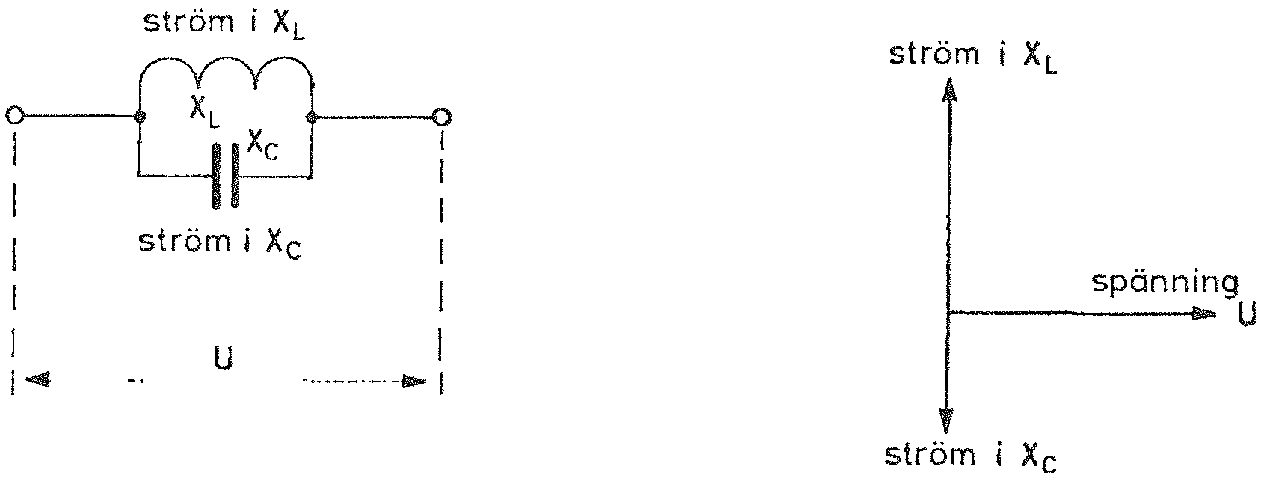
\includegraphics[width=0.8\textwidth]{images/bild_2_3-15}
\end{figure}

\begin{itemize}
  \item Reaktansen för en induktor är $X_L = 2\pi f L$
  \item Reaktansen för en kondensator är $X_C = \frac{1}{2\pi f C}$
  \item Reaktansen blir $\frac{1}{X_{LC}} = \frac{1}{X_L} - \frac{1}{X_C}$ $X_{LC}=-\frac{X_LX_C}{X_C-X_L}$
  \item Vid resonansfrekvens $f_0$, är reaktansen för bägge lika stor och tar ut varandra, varvid reaktansen går mot oändlig
  \item Resonansfrekvensen är $f_0 = \frac{1}{2\pi\sqrt{LC}}$
  \end{itemize}
\end{frame}

\begin{frame}{Serieresonanskrets}

\begin{figure}[h]
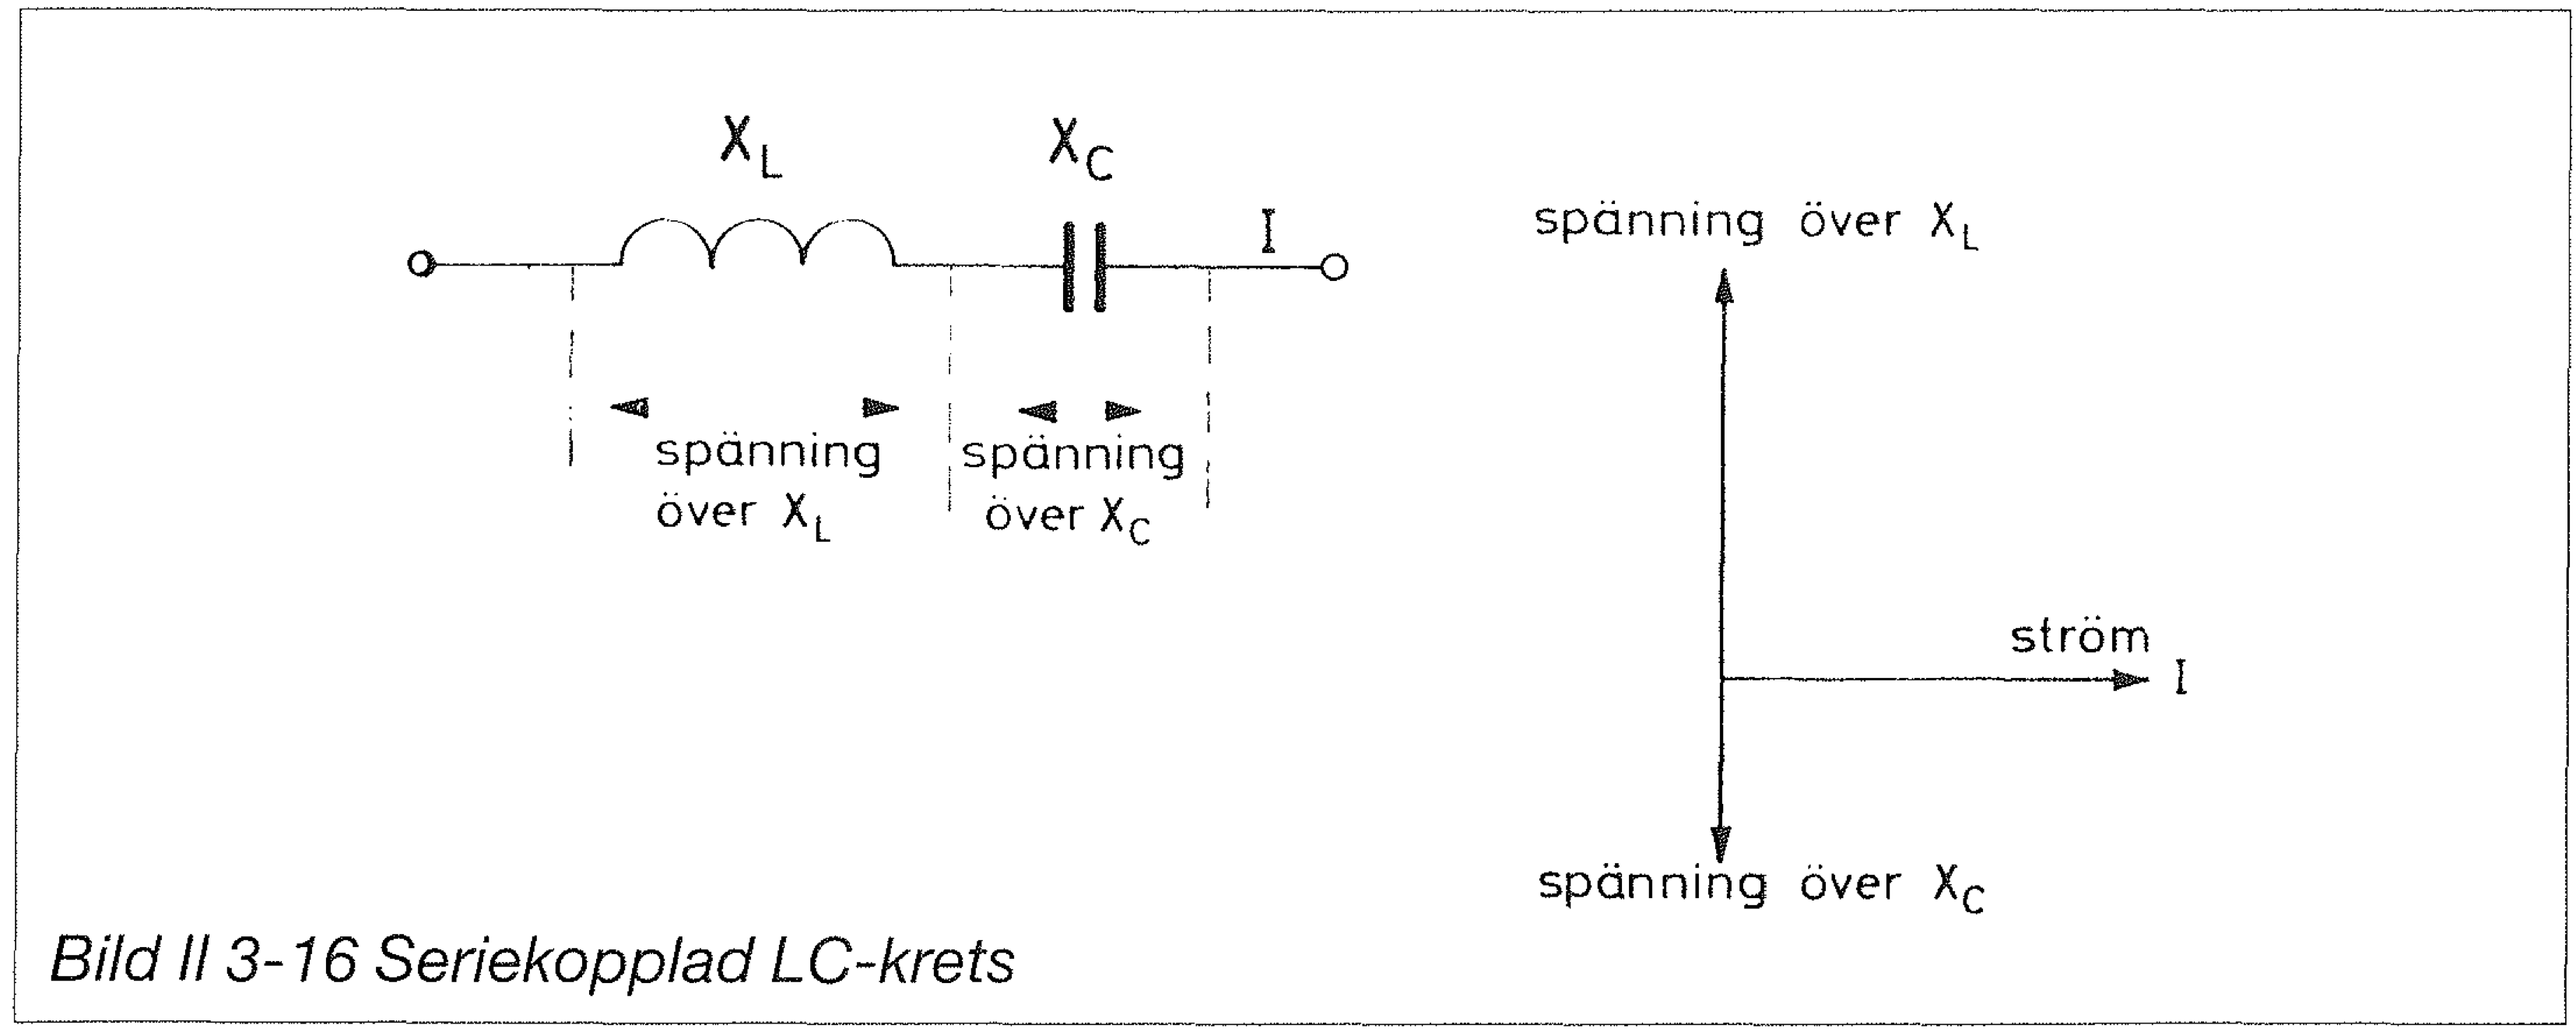
\includegraphics[width=0.8\textwidth]{images/bild_2_3-16}
\end{figure}

\begin{itemize}
  \item Reaktansen för en induktor är $X_L = 2\pi f L$
  \item Reaktansen för en kondensator är $X_C = \frac{1}{2\pi f C}$
  \item Reaktansen blir $X_{LC} = X_L - X_C$
  \item Vid resonansfrekvens $f_0$, är reaktansen för bägge lika stor och tar ut varandra, varvid reaktansen går mot noll
  \item Resonansfrekvensen är $f_0 = \frac{1}{2\pi\sqrt{LC}}$
  \end{itemize}
\end{frame}

\begin{frame}{Resonanskrets och Q-värde}

\begin{figure}[h]
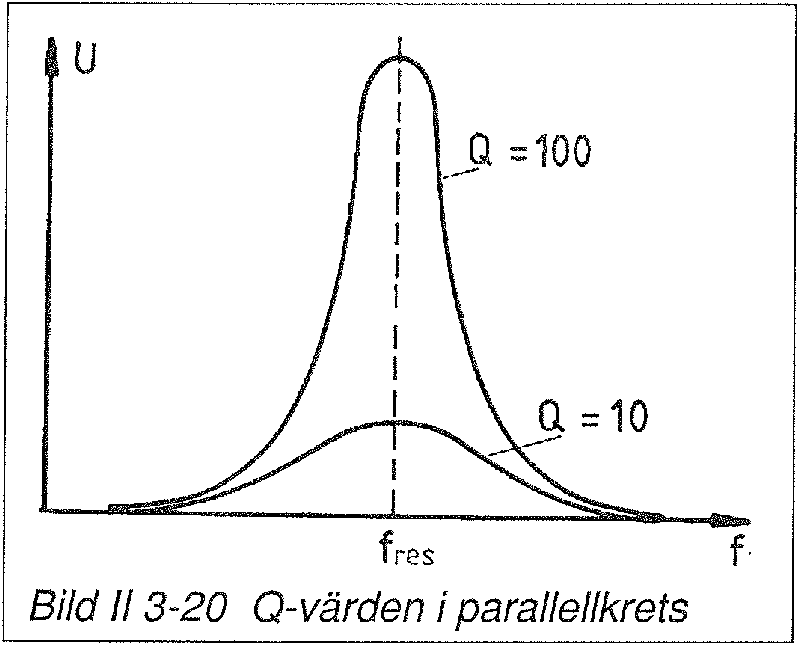
\includegraphics[width=0.4\textwidth]{images/bild_2_3-20}
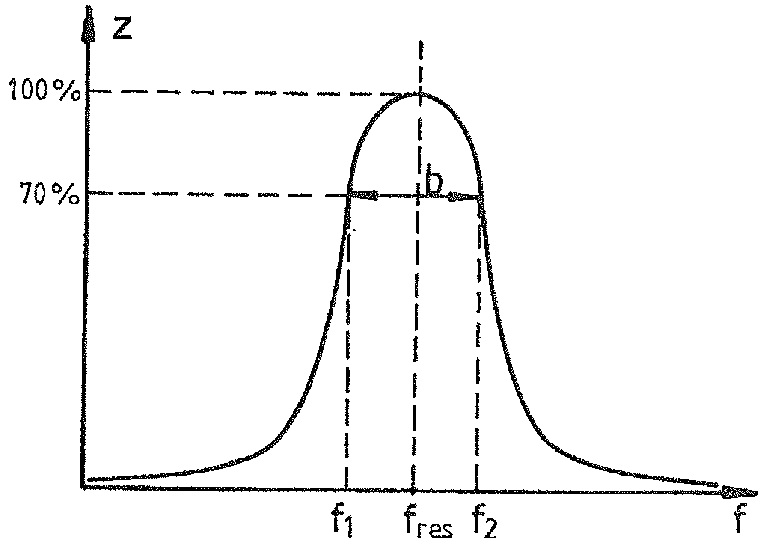
\includegraphics[width=0.4\textwidth]{images/bild_2_3-21}
\end{figure}

\begin{itemize}
  \item Godhetstalet Q (Quality factor) är en indikation på hur skarp en resonans är
  \item Energidefinition $Q = 2π\frac{\text{lagrad energi i kretsen}}{\text{energiförlusten per period}}$
    \item Bandbredden $b = f_2-f_1$
  \item Bandbreddsdefinition $Q = \frac{f_{res}}{b} = \frac{f_{res}}{f_2-f_1}$
  \end{itemize}
\end{frame}

\begin{frame}{Kvartskristall}

\begin{figure}[h]
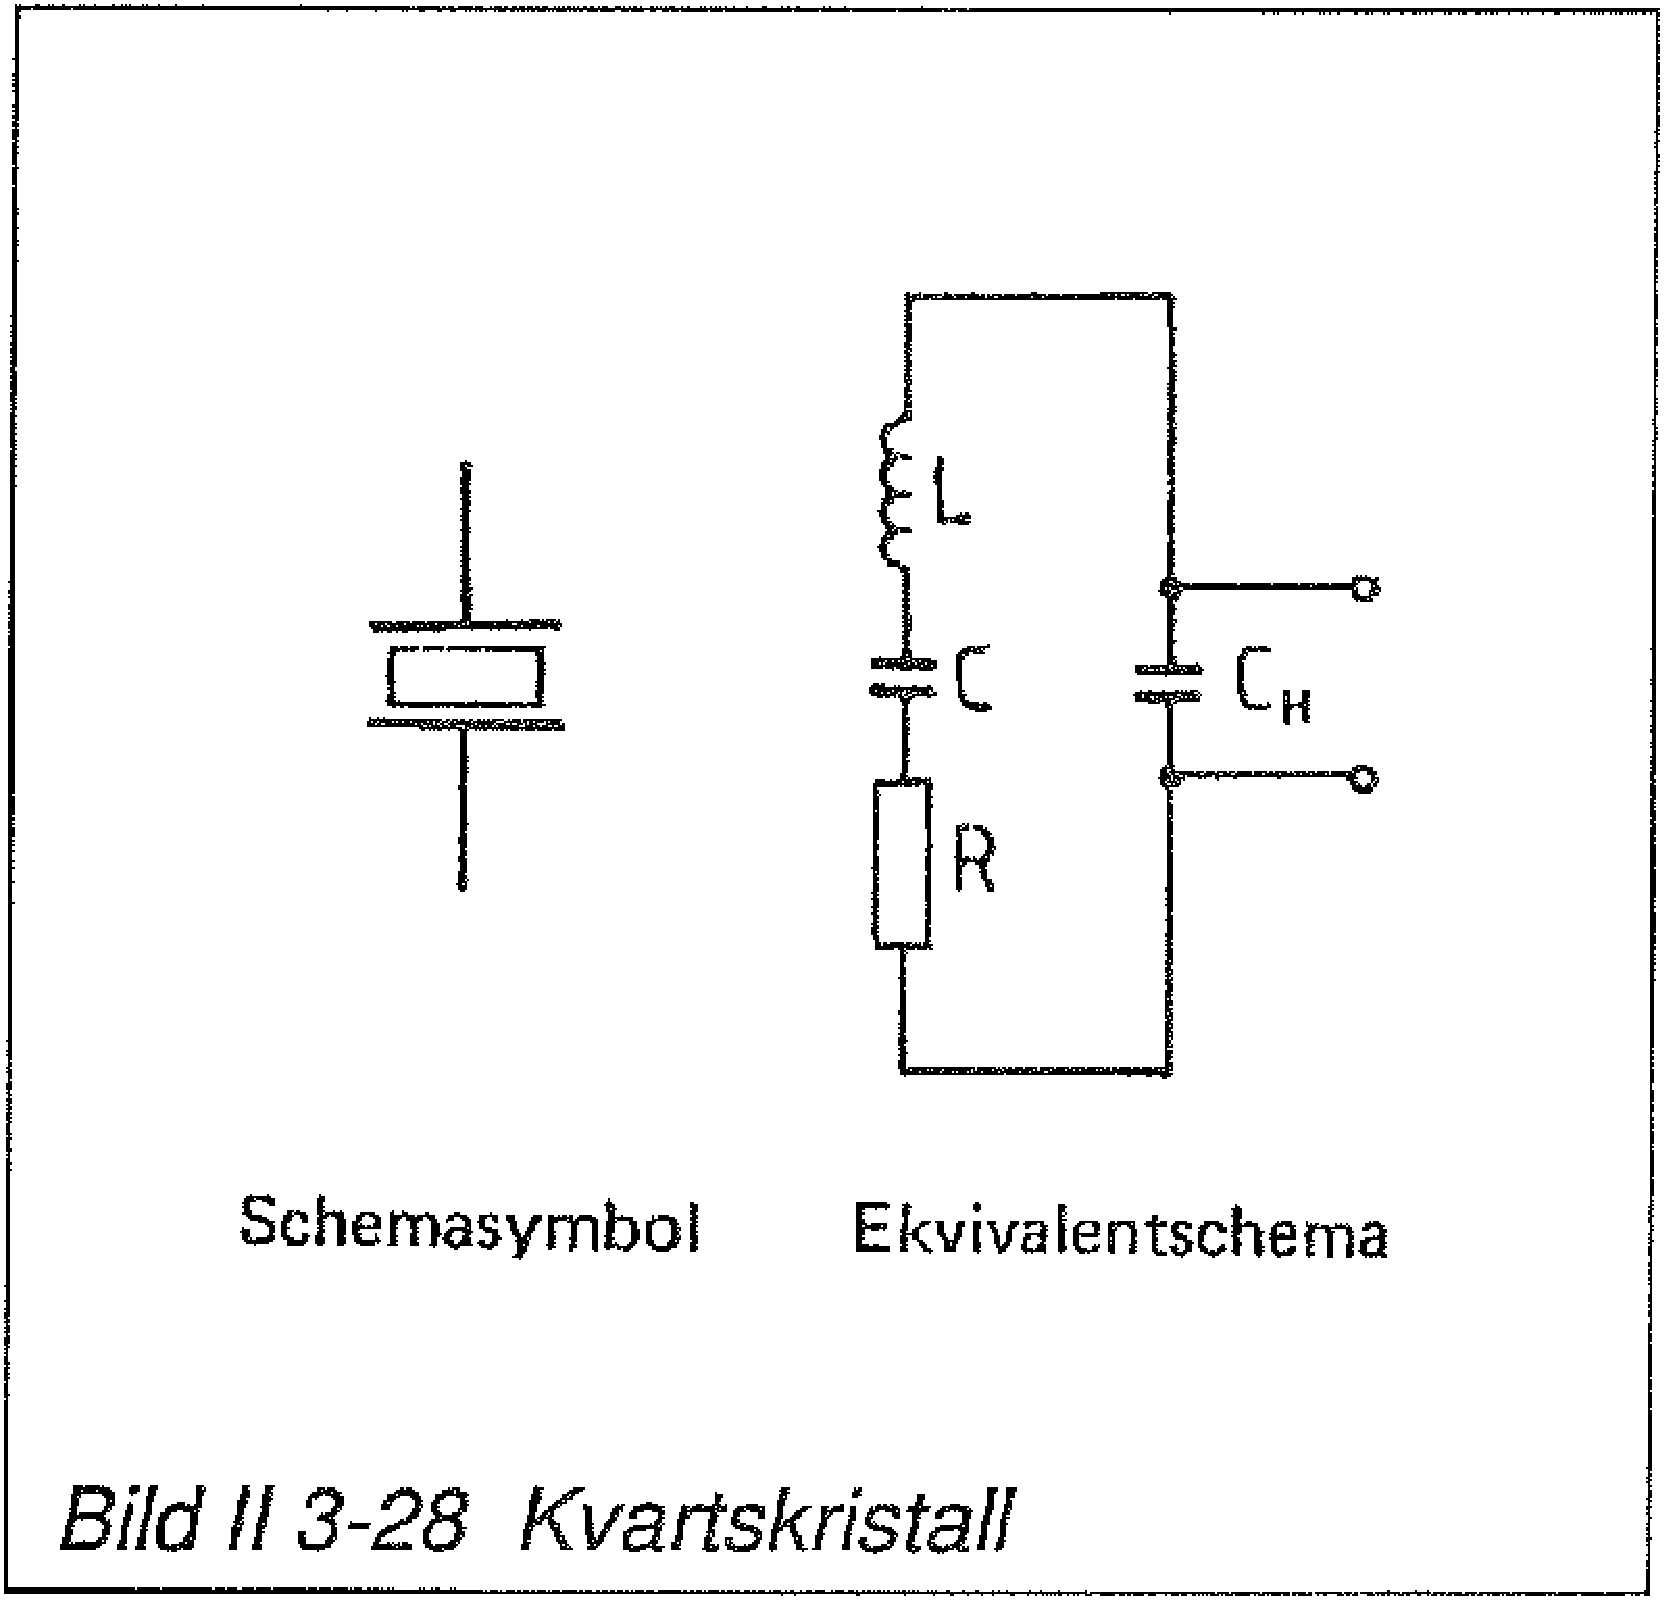
\includegraphics[width=0.4\textwidth]{images/bild_2_3-28}
\end{figure}

\begin{itemize}
  \item Kvarts ändrar form av elektrostatiska fält
  \item En kvartskristall kan aggera som en akustisk resonator
  \item Q-värden i 10000-3000000 området, oftast 100000
  \item Hyfsat stabil frekvens
  \item Frekvensen kan stabiliseras antingen med temperaturkompensering eller ungskompensering
\end{itemize}
\end{frame}

\section{Transformator}

\begin{frame}{Transformator}

\begin{figure}[h]
%  \begin{mdframed}
    \begin{center}
      \begin{circuitikz}
        \draw
        (1,1) node[transformer](T1) {}
        (T1.base) node{1}
        ;
        \draw[european]
        (4,1) node[transformer](T2) {}
        (T2.base) node{2}
        ;
        \draw
        (7,1) node[transformer core](T3) {}
        (T3.base) node{3}
        ;
      \end{circuitikz}
      \\
      \begin{tabular}{ll}
        1, 2 & Allmänna symboler \\
        3 & Transformator med kärna
      \end{tabular}
    \end{center}
    \caption{Schemasymboler för transformatorer}
%  \end{mdframed}
  \label{fig:BildII2-5}
\end{figure}

\begin{itemize}
  \item Magnetisk koppling mellan två (eller fler) spolar
  \item Galvansisk (lågfrekvent) isolation mellan kretsar
  \item Primärsidan har $n_1$ varv och sekundärsidan har $n_2$ varv
  \item Spänningsomsättning $\frac{U_1}{U_2} = \frac{n_1}{n_2}$
  \item Strömomsättning $\frac{I_1}{I_2} = \frac{n_2}{n_1}$
\end{itemize}
\end{frame}

\end{document}
